\documentclass[xcolor=dvipsnames]{beamer}
%\usepackage[czech]{babel}
\usepackage[utf8]{inputenc}
\usepackage[T1]{fontenc}

%balíček na A4
\usepackage{amsthm}
\usepackage{amsmath}
\usepackage{amsbsy}
\usepackage{amssymb}

\usepackage{graphicx}
\usepackage{lmodern}
%\usepackage{mathpazo}
\usepackage{sansmathfonts}
%\usepackage[mathlf,textlf]{MyriadPro}
%\usepackage{mathpazo}
\usepackage[small]{eulervm}
%\usepackage{newtxmath}

\usepackage{mathtools}
\usepackage{booktabs}
%\usepackage{caption}
%\usepackage{subcaption}
\usepackage{setspace}
\usepackage{array}
\usepackage{tabularx}
\usepackage{pbox}
\usepackage{mathpartir} %proof trees
\usepackage{listings}
\usepackage{xcolor}

\usepackage{tikz}
\tikzset{
   invisible/.style={opacity=0},
   visible on/.style={alt=#1{}{invisible}},
   blank/.style={},
   red on/.style={alt={#1{fill=red!10}{blank}}},
   alt/.code args={<#1>#2#3}{%
     \alt<#1>{\pgfkeysalso{#2}}{\pgfkeysalso{#3}} % \pgfkeysalso doesn't change the path
   },
 }
\usetikzlibrary{shapes.geometric,shapes.arrows,decorations.pathmorphing}
\usetikzlibrary{matrix,chains,scopes,positioning,arrows,fit}
\usetikzlibrary{automata,arrows}

%\captionsetup{compatibility=false}
%\renewcommand{\arraystretch}{1}
%\hypersetup{pdfpagemode={FullScreen}}

\makeatletter
    \newenvironment{withoutheadline}{
        \setbeamertemplate{headline}[default]
        \def\beamer@entrycode{\vspace*{-\headheight}}
    }{}
\makeatother


\title{Fairness Modulo Theory: A New Approach to LTL Software Model Checking}
\author{Daniel Dietsch, Matthias Heizmann, Vincent Langenfeld, and Andreas Podelski\vspace{-0.3cm}}
\institute{Presented by Henrich Lauko \vspace{1cm}}
\date{\today}

\usetheme{Antibes}
\setbeamertemplate{headline}{}
\setbeamertemplate{navigation symbols}{}%remove navigation symbols

\setbeamertemplate{footline}[frame number]

\definecolor{foreground}{RGB}{255,255,255}
\definecolor{background}{RGB}{24,24,24}
% \definecolor{title}{RGB}{107,174,214}
\definecolor{title}{RGB}{255,255,255}
\definecolor{main}{RGB}{39,66,96}
\definecolor{gray}{RGB}{155,155,155}
\definecolor{subtitle}{RGB}{102,255,204}
\definecolor{hilight}{RGB}{233,140,5}
\definecolor{vhilight}{RGB}{251,95,37}

\setbeamercolor{titlelike}{fg=title,bg=main}
\setbeamercolor{subtitle}{fg=subtitle}
\setbeamercolor{institute}{fg=gray}
%\setbeamercolor{normal text}{fg=foreground,bg=background}

\setbeamercolor*{block title}{fg=white, bg=main}
\setbeamercolor*{block body}{fg=black, bg=main!5}
\setbeamercolor*{block title example}{fg=white, bg=vhilight!65}
\setbeamercolor*{block body example}{fg=black, bg=vhilight!10}

\setbeamercolor{item}{fg=main} % color of bullets
%\setbeamercolor{subitem}{fg=gray}
\setbeamercolor{alerted text}{fg=hilight}
\setbeamercolor{description item}{fg=hilight}
%\setbeamercolor{itemize/enumerate subbody}{fg=gray}
\setbeamertemplate{itemize subitem}{{\textendash}}
\setbeamerfont{itemize/enumerate subbody}{size=\small}
\setbeamerfont{itemize/enumerate subitem}{size=\small}

\DeclareSymbolFont{operators}{\encodingdefault}{ppl}{m}{n}
\DeclareMathAlphabet{\mathbf}{\encodingdefault}{ppl}{bx}{n}
\DeclareMathAlphabet{\mathit}{\encodingdefault}{ppl}{m}{it}

\let\otp\titlepage
\renewcommand{\titlepage}{\otp\addtocounter{framenumber}{-1}}

\lstset{ %this is the stype
        mathescape=true,
        frame=tB,
        numbers=left,
        numberstyle=\tiny,
        basicstyle={\ttfamily\scriptsize},
        keywordstyle=\color{hilight}\bfseries,
        keywords={martin, assert, int, or, do, forall, then, let,  input, output, return, datatype, function, in, if, else, foreach, while, begin, end, SAT, UNSAT, CONFLICT, } %add the keywords you want, or load a language as Rubens explains in his comment above.
        numbers=left,
        xleftmargin=.04\textwidth,
		escapeinside={<@}{@>}
    }

\newcommand{\sat}{\textcolor{Green}}
\newcommand{\unsat}{\textcolor{Red}}

\newcommand\Wider[2][3em]{%
\makebox[\linewidth][c]{%
  \begin{minipage}{\dimexpr\textwidth+#1\relax}
  \raggedright#2
  \end{minipage}%
  }%
}

\renewcommand*{\ttdefault}{qcr}

\begin{document}

\begin{frame}[plain]
 \titlepage
\end{frame}
\section{Intro}

\section{Ultimate Automizer}
\begin{frame}
	\frametitle{Talk outline}
    \begin{enumerate}[<+->]
            \item Ultimate Automizer algorithm
            \item Reachability solving
            \item Interpolants and infeasibility proofs
            \item LTL model checking
    \end{enumerate}
\end{frame}
\begin{frame}[t,fragile]
    \frametitle{Ultimate Automizer}

    \begin{block}{Programs as languages}
        A program defines a language over program statements.
    \end{block}

    \begin{itemize}
        \item \alert{alphabet} = the set of program statements
        \item \alert{finite automaton} = control flow graph
        \item \alert{accepting states} = error locations
    \end{itemize}

	\pause
	\bigskip
	\hspace{7mm}
	\begin{minipage}{0.5\linewidth}
\begin{lstlisting}
int z:=0;
int x:=0;
while(x<20){
    if(i!=0){
        z++;
    }
    x++;
}
assert(z<=5)
\end{lstlisting}
  	\end{minipage}

	\begin{tikzpicture}[remember picture,overlay,
      trans/.style={->,>=stealth',line width=1},
      etrans/.style={->,>=stealth',line width=1,red},
      thick,inner sep=2pt,node distance=12mm,
      transHighlighted/.style={->,>=stealth',thick,red,dashed, line width=2},
      ]
      \small
      \node[xshift=-30mm,yshift=-40mm] (0) at
        (current page.north east) [circle,draw] {0};
      \node (1) [below of=0,circle,draw] {1};
      \node (2) [below of=1,circle,draw] {2};
      \node (3) [below of=2,circle,draw] {3};
      \node (4) [below of=3,xshift=-8mm,circle,draw] {4};
      \node (5) [below of=3,xshift=8mm,circle,draw] {5};
      \node (6) [right of=2,xshift=7mm,circle,draw] {6};
      \node (e) [below of=6,circle,draw,inner sep=1.6,accepting] {Err};
      \node (a) [above of=0,yshift=-5mm] {};

      \draw [trans] (a) to node {} (0);
      \draw [trans] (0) to node [right] {\texttt{z:=0}} (1);
      \draw [trans] (1) to node [right,yshift=1mm] {\texttt{x:=0}} (2);
      \draw [trans] (2) to node [above] {\texttt{x>=20}} (6);
      \draw [trans] (2) to node [right] {\texttt{x<20}} (3);
      \draw [trans] (3) to node [left,yshift=1mm] {\texttt{i=0}} (4);
      \draw [trans] (3) to node [right,yshift=1mm] {\texttt{i!=0}} (5);
      \draw [trans] (5) to node [below] {\texttt{z++}} (4);
      \draw [trans,bend left=80pt] (4) to node [left,overlay] {\texttt{x++}} (2);
      \draw [trans] (6) to node [right] {\texttt{z>5}} (e);
  \end{tikzpicture}
\end{frame}

\begin{frame}
	\frametitle{Automizer algorithm}
  \begin{center}
    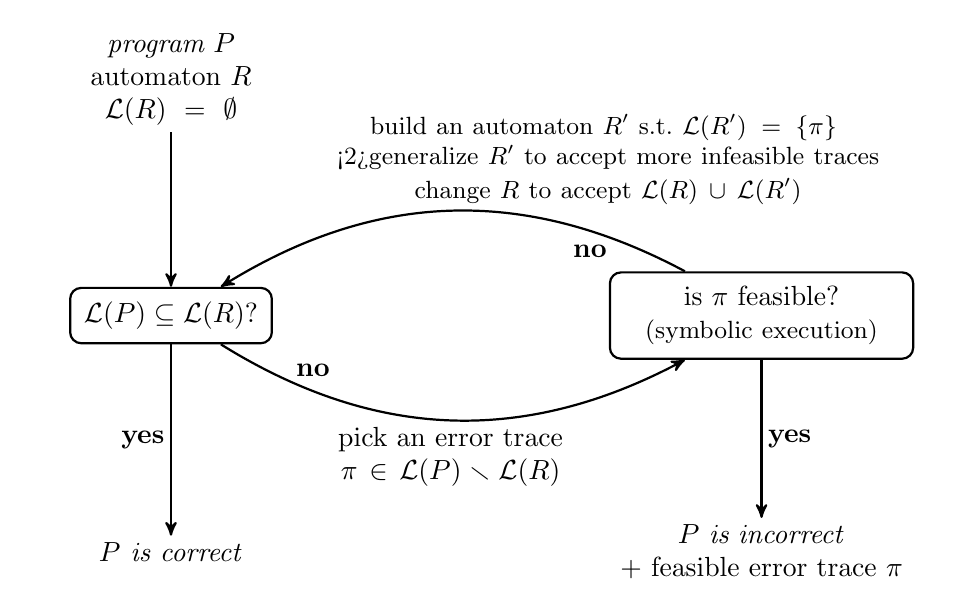
\begin{tikzpicture}[->,>=stealth',thick,inner sep=2pt,node distance=30mm,
      dn/.style={draw,rounded corners,rectangle,inner sep=5pt},
%      transHighlighted/.style={->,>=stealth,thick,red,dashed, line width=2},
      ]
      \node (P) at (0,0) [text width=35mm,align=center] {\emph{program $P$}\\
        automaton $R$\\ $\mathcal{L}(R)=\emptyset$};
      \node[dn] (check) [below of=P] {$\mathcal{L}(P)\subseteq \mathcal{L}(R)$?};
      \node (correct) [below of=check] {\emph{$P$ is correct}};
      \node[dn] (symex) [right of=check,xshift=45mm,text width=35mm,align=center]
        {is $\pi$ feasible?\\\small (symbolic execution)};
      \node (bug) [below of=symex,text width=45mm,align=center]
        {\emph{$P$ is incorrect}\\ + feasible error trace $\pi$};

      \draw (P) to node {} (check);
      \draw (check) to node[left] {\textbf{yes}} (correct);
      \draw [bend right] (check) to node[above,pos=.2,yshift=1mm] {\textbf{no}}
        node[below,text width=35mm,align=center]
        {pick an error trace\\ $\pi\in \mathcal{L}(P)\smallsetminus \mathcal{L}(R)$} (symex);
      \draw (symex) to node[right] {\textbf{yes}} (bug);
      \draw [bend right] (symex) to node[below,pos=.2,yshift=-1mm] {\textbf{no}}
        node[above,text width=75mm,align=center,xshift=20mm]
        {\small build an automaton $R'$ s.t.~$\mathcal{L}(R')=\{\pi\}$ \strut\\
         \alert<2>{generalize $R'$ to accept more infeasible traces}\\
         change $R$ to accept $\mathcal{L}(R)\cup \mathcal{L}(R')$} (check);
    \end{tikzpicture}
  \end{center}
\end{frame}

\begin{frame}
	\frametitle{Generalizition of infeasible paths}

	\begin{block}{Craig's interpolants}
	Let $\varphi,\psi$ be two first-order formulae such that $\varphi\implies\psi$.
    Then there exists a first order-formula \alert{$\theta$} called \alert{\emph{interpolant}} such that
    \begin{itemize}
    \item all non-logical symbols in \alert{$\theta$} occur in both $\varphi$ and $\psi$,
    \item $\varphi\implies\alert{\theta}\implies\psi$.
    \end{itemize}
    \end{block}

\only<1-2>{
    \begin{center}
      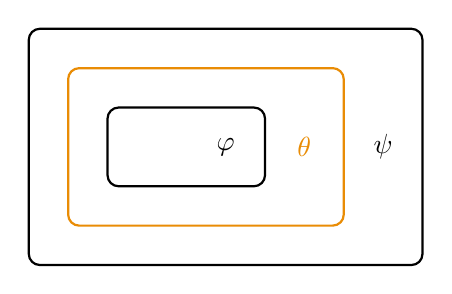
\begin{tikzpicture}[thick,rounded corners]
        \draw (0,0) rectangle (5,3);
        \draw (1,1) rectangle (3,2);
        \node at (2.5,1.5) {$\varphi$};
        \node at (4.5,1.5) {$\psi$};
        \only<2>{
          \draw[hilight] (.5,.5) rectangle (4,2.5);
          \node[hilight] at (3.5,1.5) {$\theta$}; }
      \end{tikzpicture}
    \end{center}
    }
    \only<3-4>{
    \begin{center}
      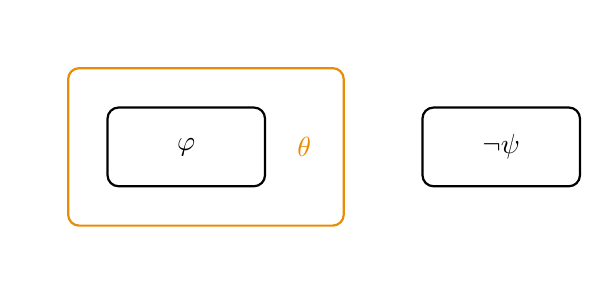
\begin{tikzpicture}[thick,rounded corners]
        \draw[white] (0,0) rectangle (7,3);
        \draw (5,1) rectangle (7,2);
        \draw (1,1) rectangle (3,2);
        \node at (2,1.5) {$\varphi$};
        \node at (6,1.5) {$\neg\psi$};
        \only<4>{
          \draw[hilight] (.5,.5) rectangle (4,2.5);
          \node[hilight] at (3.5,1.5) {$\theta$};
        }
      \end{tikzpicture}
    \end{center}
    }

\end{frame}

\begin{frame}[fragile]
	\frametitle{Example: Error path}

  \begin{tabular}{cp{1ex}c}
  \begin{minipage}{.40\linewidth}
      \begin{minipage}{.90\linewidth}
\begin{lstlisting}
int z:=0;
int x:=0;
while(x<20){
    if(i!=0){
        z++;
    }
    x++;
}
assert(z<=5)
\end{lstlisting}
      \end{minipage}
 \end{minipage}
&&
 \begin{minipage}{.55\linewidth}
    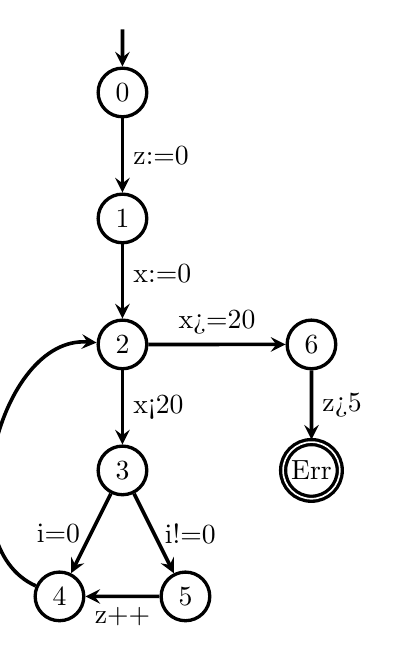
\begin{tikzpicture}[scale=0.8, trans/.style={->,>=stealth,line width=1.3},
      etrans/.style={->,>=stealth,line width=1.3,red},very thick,
      transHighlighted/.style={->,>=stealth,thick,red,dashed, line width=3},
      ]
      % \scriptsize
      \node (0) at (1,0) [circle,draw] {0};
      \node (1) at (1,-2) [circle,draw] {1};
      \node (2) at (1,-4) [circle,draw] {2};
      \node (3) at (1,-6) [circle,draw] {3};
      \node (4) at (0,-8) [circle,draw] {4};
      \node (5) at (2,-8) [circle,draw] {5};
      \node (6) at (4,-4) [circle,draw] {6};
      \node (e) at (4,-6) [circle,draw,inner sep=1.6,accepting] {Err};

      \draw [trans] (1,1) to node {} (0);
      \alert<2->{\draw [trans] (0) to node [right] {\texttt{z:=0}} (1);}
      \alert<2->{\draw [trans] (1) to node [right,yshift=1mm] {\texttt{x:=0}} (2);}
      \alert<2->{\draw [trans] (2) to node [above] {\texttt{x>=20}} (6);}
      \draw [trans] (2) to node [right] {\texttt{x<20}} (3);
      \draw [trans] (3) to node [left] {\texttt{i=0}} (4);
      \draw [trans] (3) to node [right] {\texttt{i!=0}} (5);
      \draw [trans] (5) to node [below] {\texttt{z++}} (4);
      \draw [trans,bend left=80pt,overlay] (4)
        to node [left,overlay] {\texttt{x++}} (2);
      \alert<2->{\draw [trans] (6) to node [right] {\texttt{z>5}} (e);}
    \end{tikzpicture}
  \end{minipage}
\end{tabular}
\end{frame}

\begin{frame}[fragile]
	\frametitle{Example: Error path}

  \begin{tabular}{cp{1ex}c}
  \begin{minipage}{.40\linewidth}
    \begin{center}
    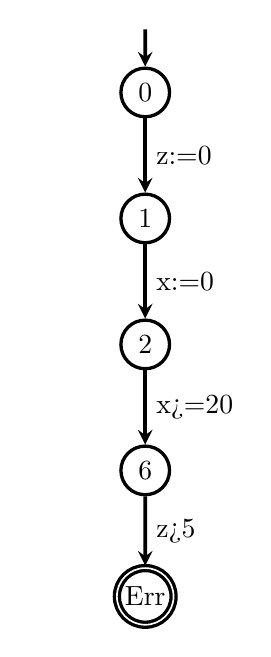
\begin{tikzpicture}[scale=0.8, trans/.style={->,>=stealth,line width=1.3},
      etrans/.style={->,>=stealth,line width=1.3,red},very thick,
      transHighlighted/.style={->,>=stealth,thick,red,dashed, line width=3},
      ]
      % \scriptsize
      \node (b) at (-.5,0) [white] {aa};
      \node (0) at (1,0) [circle,draw] {0};
      \node (1) at (1,-2) [circle,draw] {1};
      \node (2) at (1,-4) [circle,draw] {2};
      \node (6) at (1,-6) [circle,draw] {6};
      \node (e) at (1,-8) [circle,draw,inner sep=1.6,accepting] {Err};

      \draw [trans] (1,1) to node {} (0);
      \draw [trans] (0) to node [right] {\texttt{z:=0}} (1);
      \draw [trans] (1) to node [right] {\texttt{x:=0}} (2);
      \draw [trans] (2) to node [right] {\texttt{x>=20}} (6);
      \draw [trans] (6) to node [right] {\texttt{z>5}} (e);
    \end{tikzpicture}
    \end{center}
 \end{minipage}
&&
 \begin{minipage}{.40\linewidth}
    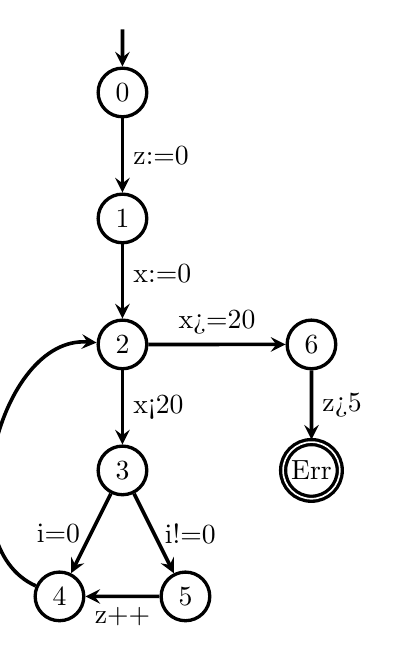
\begin{tikzpicture}[scale=0.8, trans/.style={->,>=stealth,line width=1.3},
      etrans/.style={->,>=stealth,line width=1.3,red},very thick,
      transHighlighted/.style={->,>=stealth,thick,red,dashed, line width=3},
      ]
      % \scriptsize
      \node (0) at (1,0) [circle,draw] {0};
      \node (1) at (1,-2) [circle,draw] {1};
      \node (2) at (1,-4) [circle,draw] {2};
      \node (3) at (1,-6) [circle,draw] {3};
      \node (4) at (0,-8) [circle,draw] {4};
      \node (5) at (2,-8) [circle,draw] {5};
      \node (6) at (4,-4) [circle,draw] {6};
      \node (e) at (4,-6) [circle,draw,inner sep=1.6,accepting] {Err};

      \draw [trans] (1,1) to node {} (0);
      \alert{\draw [trans] (0) to node [right] {\texttt{z:=0}} (1);}
      \alert{\draw [trans] (1) to node [right,yshift=1mm] {\texttt{x:=0}} (2);}
      \alert{\draw [trans] (2) to node [above] {\texttt{x>=20}} (6);}
      \draw [trans] (2) to node [right] {\texttt{x<20}} (3);
      \draw [trans] (3) to node [left] {\texttt{i=0}} (4);
      \draw [trans] (3) to node [right] {\texttt{i!=0}} (5);
      \draw [trans] (5) to node [below] {\texttt{z++}} (4);
      \draw [trans,bend left=80pt,overlay] (4)
        to node [left,overlay] {\texttt{x++}} (2);
      \alert{\draw [trans] (6) to node [right] {\texttt{z>5}} (e);}
    \end{tikzpicture}
  \end{minipage}
\end{tabular}
\end{frame}
\begin{frame}
    \only<1>{\frametitle{Error feasibility analysis}}
    \only<2->{\frametitle{Generalization of infeasible trace}}
\begin{tabular}{cp{1ex}c}
  \begin{minipage}{.35\linewidth}
    \begin{center}
    \begin{tikzpicture}[scale=0.8, trans/.style={->,>=stealth,line width=1.3},
      etrans/.style={->,>=stealth,line width=1.3,red},thick,
      transHighlighted/.style={->,>=stealth,thick,red,dashed, line width=3},
      ]
      % \scriptsize
      \node (b) at (-.5,0) [white] {};
      \node (0) at (1,0) [circle,draw] {0};
      \node (1) at (1,-2) [circle,draw] {1};
      \node (2) at (1,-4) [circle,draw] {2};
      \node (6) at (1,-6) [circle,draw] {6};
      \node (e) at (1,-8) [circle,draw,inner sep=1.6,accepting] {Err};

      \draw [trans] (1,1) to node {} (0);
      \draw [trans] (0) to node [right] {\texttt{z:=0}} (1);
      \draw [trans] (1) to node [right] {\texttt{x:=0}} (2);
      \draw [trans] (2) to node [right] {\texttt{x>=20}} (6);
      \draw [trans] (6) to node [right] {\texttt{z>5}} (e);

        \only<3->{\node (l0) at (-0.2,0) [hilight] {$\mathrm{true}$};}
      \only<5->{\node (l0) at (-0.2,-2) [hilight] {$z=0$};}
      \only<7->{\node (l0) at (-0.2,-4) [hilight] {$z=0$};}
      \only<9->{\node (l0) at (-0.2,-6) [hilight] {$z=0$};}
        \only<11->{\node (l0) at (-0.2,-8) [hilight] {$\mathrm{false}$};}
    \end{tikzpicture}
    \end{center}
  \end{minipage}
&&
  \begin{minipage}{.55\linewidth}
    \only<1>{
      Symbolic execution produces:
	  \[
		z=0 ~\wedge~ x=0 ~\wedge~ x \geq 20 ~\wedge~ z>5 \equiv\mathrm{false}
	  \]
      So the error trace is \alert{\emph{infeasible}}.
    }
    \only<2-11>{
      \begin{tikzpicture}[thick,rounded corners]
        \draw[white] (.5,-.5) rectangle (5.5,-4);
        \draw (1,-1) rectangle (5,-3);
          \only<2-3>{\node at (3,-2) {$\mathrm{true}$};}
          \only<4-5>{\node at (3,-2) {\alert{$\mathrm{true}$}$~\land~z=0$};}
          \only<6-7>{\node at (3,-2) {\alert{$z=0$}$~\land~x=0$};}
          \only<8-9>{\node at (3,-2) {\alert{$z=0$}$~\land~x\ge20$};}
          \only<10-11>{\node at (3,-2) {\alert{$z=0$}$~\land~z>5$};}
        \draw (1,-5) rectangle (5,-7);
        \only<2-3>{\node[text width=37mm,align=center] at (3,-6)
          {$~~~~z=0~\land~x=0~\land~$\\
          $~\land~x\ge20~\land~z>5~~~~$};}
        \only<4-5>{\node[text width=37mm,align=center] at (3,-6)
          {\phantom{$~~~~z=0~\land~$}$x=0~\land~$\\
          $~\land~ x\ge20~\land~ z>5~~~~$};}
        \only<6-7>{\node[text width=37mm,align=center] at (3,-6)
          {\phantom{$~~~~z=0~\land~x=0~\land~$}\\
           \phantom{$~\land~$}$x\ge20~\land~z>5~~~~$};}
        \only<8-9>{\node[text width=37mm,align=center] at (3,-6)
          {\phantom{$~~~~z=0~\land~x=0~\land~$}\\
           \phantom{$~\land~x\ge20~\land~$}$z>5~~~~$};}
        \only<10-11>{\node[text width=37mm,align=center] at (3,-6)
          {$true$};}
        \only<3,5,7,9,11>{\draw[hilight] (.5,-.5) rectangle (5.5,-4);}
          \only<3>{\node[hilight] at (3,-3.5) {$\mathrm{true}$};}
        \only<5,7,9>{\node[hilight] at (3,-3.5) {$z=0$};}
          \only<11>{\node[hilight] at (3,-3.5) {$\mathrm{false}$};}
      \end{tikzpicture}
    }
	\only<12->{
      \begin{tikzpicture}[scale=0.8, trans/.style={->,>=stealth,line width=1.3},
          etrans/.style={->,>=stealth,line width=1.3,red},very thick,
          transHighlighted/.style={->,>=stealth,thick,red,dashed, line width=3},
        ]
        % \scriptsize
        \node (0) at (1,0) [circle,draw,hilight] {$\mathrm{true}$};
        \node (1) at (1,-3) [circle,draw,hilight] {$z=0$};
        \node (2) at (1,-6) [circle,draw,hilight,accepting] {$\mathrm{false}$};

       \only<12>{ \draw [trans,white] (-.5,0) to (0);}
       \only<13->{ \draw [trans] (-.5,0) to (0);}
       \only<13->{ \draw [trans,loop right] (0) to node [right]
          {$\Sigma\setminus\{\texttt{z:=0}\}$} (0);}
        \only<13->{ \draw [trans] (0) to node [right] {\texttt{z:=0}} (1); }
        \only<14->{ \draw [trans,loop right] (1) to node [right]
          {$\Sigma\setminus\{\texttt{z++},~\texttt{z>5}\}$} (1);}
        \only<15->{ \draw [trans] (1) to node [right] {\texttt{z>5}} (2); }
        \only<15->{ \draw [trans,bend left,overlay] (1) to node [left,overlay]
          {\texttt{z++}} (0); }
        \only<16->{ \draw [trans,loop right] (2) to node [right] {$\Sigma$} (2);}
      \end{tikzpicture}

      \bigskip
      \begin{overlayarea}{1.0\linewidth}{10mm}
          $\Sigma=\{$\texttt{z:=0}, \texttt{x:=0}, \texttt{x>=20}, \texttt{x<20},\\
        $~~~~~~~~$\texttt{i=0}, \texttt{i!=0}, \texttt{z++},
        \texttt{x++}, \texttt{z>5}$\}$
      \end{overlayarea}
    }
  \end{minipage}
\end{tabular}
\end{frame}

\begin{frame}
	\frametitle{Automizer algorithm}
  \begin{center}
    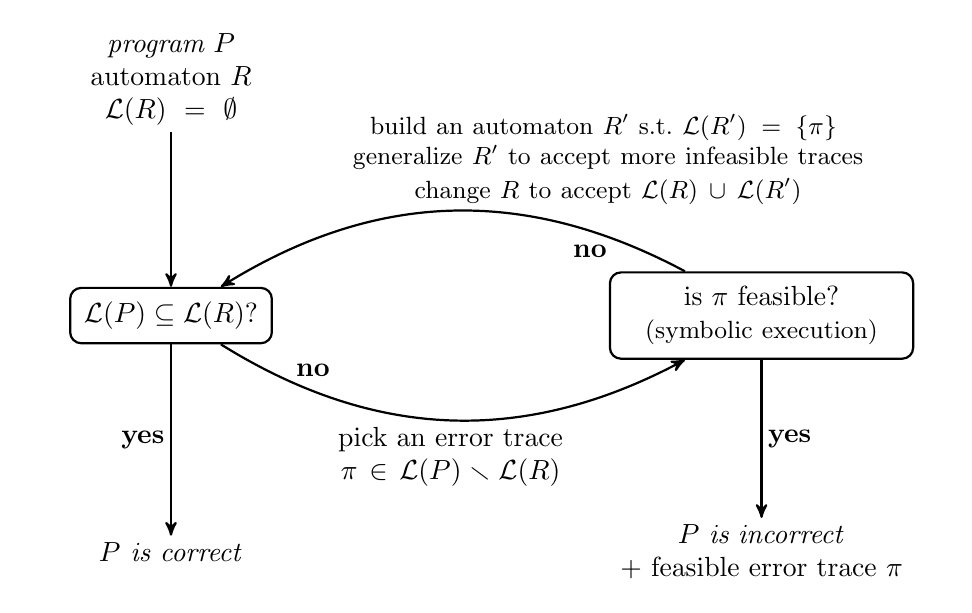
\begin{tikzpicture}[->,>=stealth',thick,inner sep=2pt,node distance=30mm,
      dn/.style={draw,rounded corners,rectangle,inner sep=5pt},
%      transHighlighted/.style={->,>=stealth,thick,red,dashed, line width=2},
      ]
      \node (P) at (0,0) [text width=35mm,align=center] {\emph{program $P$}\\
        automaton $R$\\ $\mathcal{L}(R)=\emptyset$};
      \node[dn] (check) [below of=P] {$\mathcal{L}(P)\subseteq \mathcal{L}(R)$?};
      \node (correct) [below of=check] {\emph{$P$ is correct}};
      \node[dn] (symex) [right of=check,xshift=45mm,text width=35mm,align=center]
        {is $\pi$ feasible?\\\small (symbolic execution)};
      \node (bug) [below of=symex,text width=45mm,align=center]
        {\emph{$P$ is incorrect}\\ $+$ feasible error trace $\pi$};

      \draw (P) to node {} (check);
      \draw (check) to node[left] {\textbf{yes}} (correct);
      \draw [bend right] (check) to node[above,pos=.2,yshift=1mm] {\textbf{no}}
        node[below,text width=35mm,align=center]
        {pick an error trace\\ $\pi\in \mathcal{L}(P)\smallsetminus \mathcal{L}(R)$} (symex);
      \draw (symex) to node[right] {\textbf{yes}} (bug);
      \draw [bend right] (symex) to node[below,pos=.2,yshift=-1mm] {\textbf{no}}
        node[above,text width=75mm,align=center,xshift=20mm]
        {\small build an automaton $R'$ s.t.~$\mathcal{L}(R')=\{\pi\}$ \strut\\
         \alert{generalize $R'$ to accept more infeasible traces}\\
         change $R$ to accept $\mathcal{L}(R)\cup \mathcal{L}(R')$} (check);
    \end{tikzpicture}
  \end{center}
\end{frame}

\begin{frame}[t]
    \frametitle{ $\mathcal{L}(P)\subseteq \mathcal{L}(R)$? }
\begin{tabular}{cp{1ex}c}
  \begin{minipage}{.35\linewidth}
	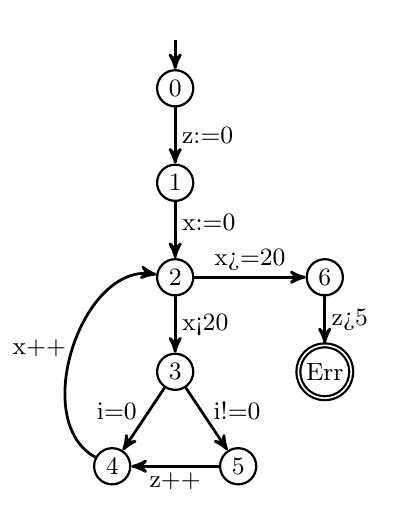
\begin{tikzpicture}[
      trans/.style={->,>=stealth',line width=1},
      etrans/.style={->,>=stealth',line width=1,red},
      thick,inner sep=2pt,node distance=12mm,
      transHighlighted/.style={->,>=stealth',thick,red,dashed, line width=2},
      ]
      \small
      \node[xshift=-30mm,yshift=-40mm] (0) at
        (current page.north east) [circle,draw] {0};
      \node (1) [below of=0,circle,draw] {1};
      \node (2) [below of=1,circle,draw] {2};
      \node (3) [below of=2,circle,draw] {3};
      \node (4) [below of=3,xshift=-8mm,circle,draw] {4};
      \node (5) [below of=3,xshift=8mm,circle,draw] {5};
      \node (6) [right of=2,xshift=7mm,circle,draw] {6};
      \node (e) [below of=6,circle,draw,inner sep=1.6,accepting] {Err};
      \node (a) [above of=0,yshift=-5mm] {};

      \draw [trans] (a) to node {} (0);
      \draw [trans] (0) to node [right] {\texttt{z:=0}} (1);
      \draw [trans] (1) to node [right,yshift=1mm] {\texttt{x:=0}} (2);
      \draw [trans] (2) to node [above] {\texttt{x>=20}} (6);
      \draw [trans] (2) to node [right] {\texttt{x<20}} (3);
      \draw [trans] (3) to node [left,yshift=1mm] {\texttt{i=0}} (4);
      \draw [trans] (3) to node [right,yshift=1mm] {\texttt{i!=0}} (5);
      \draw [trans] (5) to node [below] {\texttt{z++}} (4);
      \draw [trans,bend left=80pt] (4) to node [left,overlay] {\texttt{x++}} (2);
      \draw [trans] (6) to node [right] {\texttt{z>5}} (e);
  \end{tikzpicture}
  \end{minipage}
&&
  \begin{minipage}{.60\linewidth}
	\begin{center}
      \begin{tikzpicture}[scale=0.7, trans/.style={->,>=stealth,line width=1.3},
          etrans/.style={->,>=stealth,line width=1.3,red},very thick,
          transHighlighted/.style={->,>=stealth,thick,red,dashed, line width=3},
        ]
        % \scriptsize
        \only<1>{
            \node (0) at (1,0) [circle,draw] {$\mathrm{true}$};
            \node (1) at (1,-3) [circle,draw] {$x=0$};
            \node (2) at (1,-6) [circle,draw,accepting] {$\mathrm{false}$};
        }
        \only<2>{
            \node (0) at (1,0) [circle,draw, accepting] {$\mathrm{true}$};
            \node (1) at (1,-3) [circle,draw, accepting] {$x=0$};
            \node (2) at (1,-6) [circle,draw] {$\mathrm{false}$};
        }
        \draw [trans,white] (-.5,0) to (0);
        \draw [trans] (-.5,0) to (0);
        \draw [trans,loop right] (0) to node [right]
          {$\Sigma\setminus\{\texttt{z:=0}\}$} (0);
        \draw [trans] (0) to node [right] {\texttt{z:=0}} (1);
        \draw [trans,loop right] (1) to node [right]
          {$\Sigma\setminus\{\texttt{z++},~\texttt{z>5}\}$} (1);
        \draw [trans] (1) to node [right] {\texttt{z>5}} (2);
        \draw [trans,bend left,overlay] (1) to node [left,overlay]
          {\texttt{z++}} (0);
        \draw [trans,loop right] (2) to node [right] {$\Sigma$} (2);
      \end{tikzpicture}
	\end{center}
  \end{minipage}
\end{tabular}
    \pause
    \bigskip

    $\mathcal{L}(P)\subseteq \mathcal{L}(R)$ iff the language of the synchronous
    product of $P$ and \alert{complemented $R$} is empty.

\end{frame}

\section{LTL model checking}
\begin{frame}[t]
	\frametitle{LTL model checking}
    \begin{block}{LTL model checking problem}
        Does the program $\mathcal{P}$ \emph{satisfy} the property $\varphi$?
    \end{block}

    \pause

    \textbf{Automizer approach:}
    \begin{itemize}[<+->]
        \item LTL property $\varphi$ is represented by Büchi automaton $\mathcal{A}_\varphi$
        \item creates Büchi program $\mathcal{B} = \mathcal{P} \times \mathcal{A}_{\neg \varphi}$
        \item violation of property is proven via a feasible \emph{fair} path
    \end{itemize}

    \pause
    \begin{block}{Fair path}
        Path is fair if it visits set of accepting states infinitely often.
    \end{block}
\end{frame}
\begin{frame}[fragile]
    \frametitle{Example: Büchi program}
\begin{tabular}{cp{1ex}c}
  \begin{minipage}{.40\linewidth}
\textbf{Program:}
\begin{lstlisting}
int x, y;
while( true ){
    x := *;
    y := 1;
    while( x > 0 ){
        x--;
        if( x <= 1 )
            y := 0;
    }
}
\end{lstlisting}
\textbf{LTL property:}
\[
    \varphi \equiv G(x > 0 \implies F(y = 0))
\]
  \end{minipage}
&&
  \begin{minipage}{.55\linewidth}
    \includegraphics[width=\textwidth,height=0.5\textheight,keepaspectratio]{code.jpg} \\

    \includegraphics[width=\textwidth,height=0.35\textheight,keepaspectratio]{buchi.jpg}
  \end{minipage}
\end{tabular}
\end{frame}

\begin{frame}
    \frametitle{Example: Büchi program}
    \includegraphics[width=\textwidth,height=\textheight,keepaspectratio]{product.jpg} \\
\end{frame}

\begin{frame}
	\frametitle{Infeasible path}

    An infinite path is \alert{infeasible} if:
    \pause
    \begin{enumerate}
            \item some finite prefix is not feasible.\\
            \pause
            \bigskip
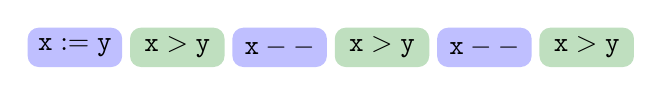
\begin{tikzpicture}[shorten >=1pt,->]
    \tikzstyle{path}=[rectangle,rounded corners,fill=blue!25,inner sep=0pt,minimum width=1.2cm,minimum height=0.5cm]
    \tikzstyle{assume}=[rectangle,rounded corners,fill=Green!25,inner sep=0pt,minimum width=1.2cm,minimum height=0.5cm]
    \node[path] (1) at (0,0) {$\mathtt{x:=y}$};
    \node[assume] (1) at (1.3,0) {$\mathtt{x>y}$};
    \node[path] (1) at (2.6,0) {$\mathtt{x--}$};
    \node[assume] (1) at (3.9,0) {$\mathtt{x>y}$};
    \node[path] (1) at (5.2,0) {$\mathtt{x--}$};
    \node[assume] (1) at (6.5,0) {$\mathtt{x>y}$};

\end{tikzpicture}
$\dots$
\pause
    \item there is a \alert{ranking function} for the path, ie. the execution is terminating.\\
    \pause
    \bigskip
\pause
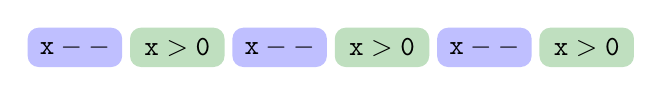
\begin{tikzpicture}[shorten >=1pt,->]
    \tikzstyle{path}=[rectangle,rounded corners,fill=blue!25,inner sep=0pt,minimum width=1.2cm,minimum height=0.5cm]
    \tikzstyle{assume}=[rectangle,rounded corners,fill=Green!25,inner sep=0pt,minimum width=1.2cm,minimum height=0.5cm]
    \node[path] (1) at (0,0) {$\mathtt{x--}$};
    \node[assume] (1) at (1.3,0) {$\mathtt{x>0}$};
    \node[path] (1) at (2.6,0) {$\mathtt{x--}$};
    \node[assume] (1) at (3.9,0) {$\mathtt{x>0}$};
    \node[path] (1) at (5.2,0) {$\mathtt{x--}$};
    \node[assume] (1) at (6.5,0) {$\mathtt{x>0}$};

\end{tikzpicture}
	$\dots$\\
\pause
    Termination proof: $r(x,y) = x$
    \end{enumerate}

    \pause
    \bigskip
\end{frame}

\begin{frame}
	\frametitle{Ultimate LTL Automizer}
    \includegraphics[width=\textwidth,height=0.9\textheight,keepaspectratio]{ltlultimate.jpg}
\end{frame}

\begin{frame}
	\frametitle{Implementation details}
    \begin{itemize}[<+->]
        \item using parser for ANSI C
        \item LTL property in ACLS format
        \item using LTL2BA
        \item own source-to-source transformations
        \item own trace abstraction, ranking function synthesis, automata manipulations
    \end{itemize}
\end{frame}

\begin{frame}
	\frametitle{Some benchmarks}
    \includegraphics[width=\textwidth,height=0.9\textheight,keepaspectratio]{table-big.jpg}
\end{frame}

\begin{frame}
	\frametitle{Some benchmarks}
    \includegraphics[width=\textwidth,height=0.9\textheight,keepaspectratio]{table-small.jpg}
\end{frame}
\section{Results}
\end{document}

%%% Local Variables:
%%% mode: latex
%%% TeX-master: t
%%% End:
